% Beamer presentation paired with paper_visual.tex.
% Reuses every PDF figure under results/figures/ -- one big visual per
% slide, basics -> advanced.  Build:  pdflatex slides.tex (twice).
\documentclass[aspectratio=169,11pt]{beamer}
\usetheme{metropolis}
\usepackage{graphicx}
\usepackage{tikz}
\usepackage{booktabs}
\usepackage{amsmath,amssymb}
\usetikzlibrary{arrows.meta,positioning,fit,shapes.geometric}
\graphicspath{{../results/figures/}}

\definecolor{accent}{HTML}{D62728}
\definecolor{ink}{HTML}{222222}
\setbeamercolor{frametitle}{fg=accent}
\setbeamercolor{title}{fg=accent}

\title{FOCUS: A 400K-Parameter\\Cross-Attention Assigner for Receipt KIE}
\subtitle{End-to-end vs.\ pipeline on SROIE}
\author{Anonymous}
\date{Conference 2026 (under review)}

\begin{document}

\begin{frame}\titlepage\end{frame}

% ---------------------------------------------------------------
\begin{frame}{The 30-second pitch}
\begin{columns}[T]
\column{0.46\textwidth}
\textbf{Problem.} Pull \textsf{company / date / address / total} from
receipt images.

\medskip
\textbf{Two paradigms.}
\begin{itemize}
  \item \textbf{End-to-end (DONUT)} -- 200M params, opaque.
  \item \textbf{Pipeline} -- detect + read + assign, interpretable.
\end{itemize}

\medskip
\textbf{Our claim.} A \textbf{400K}-parameter \emph{assigner} closes the
F1 gap to DONUT, exposes per-field attention, and is calibrated.

\column{0.50\textwidth}
\centering
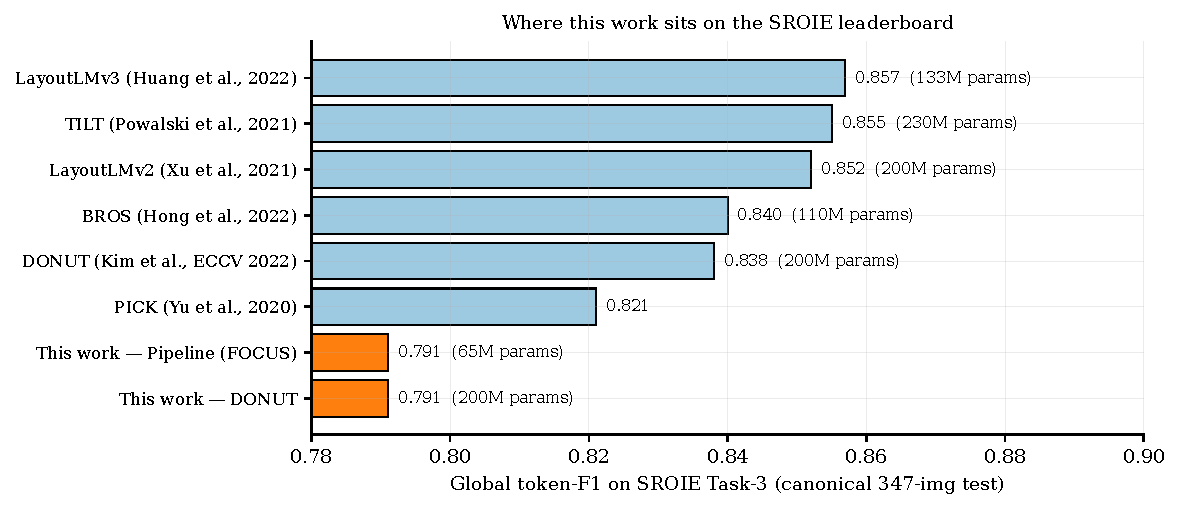
\includegraphics[width=\linewidth]{fig_competitors.pdf}
\end{columns}
\end{frame}

% ---------------------------------------------------------------
\begin{frame}{What is the assigner? (basic)}
\begin{columns}[T]
\column{0.45\textwidth}
\begin{itemize}
  \item Receipt $\to$ $\sim$24 OCR tokens.
  \item Pick the right token for each of 4 fields.
  \item That's it. No magic.
\end{itemize}
\bigskip
\emph{Question:} how do we teach a model to make 4 picks from a bag of
words?
\column{0.50\textwidth}
\centering
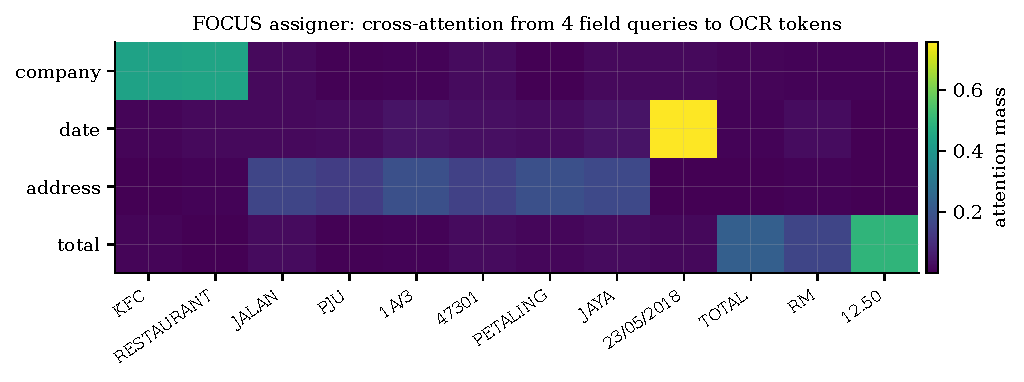
\includegraphics[width=\linewidth]{fig_attention_heatmap.pdf}\\
\scriptsize Real cross-attention from 4 queries to OCR tokens.
\end{columns}
\end{frame}

% ---------------------------------------------------------------
\begin{frame}{How it works (intermediate)}
\centering
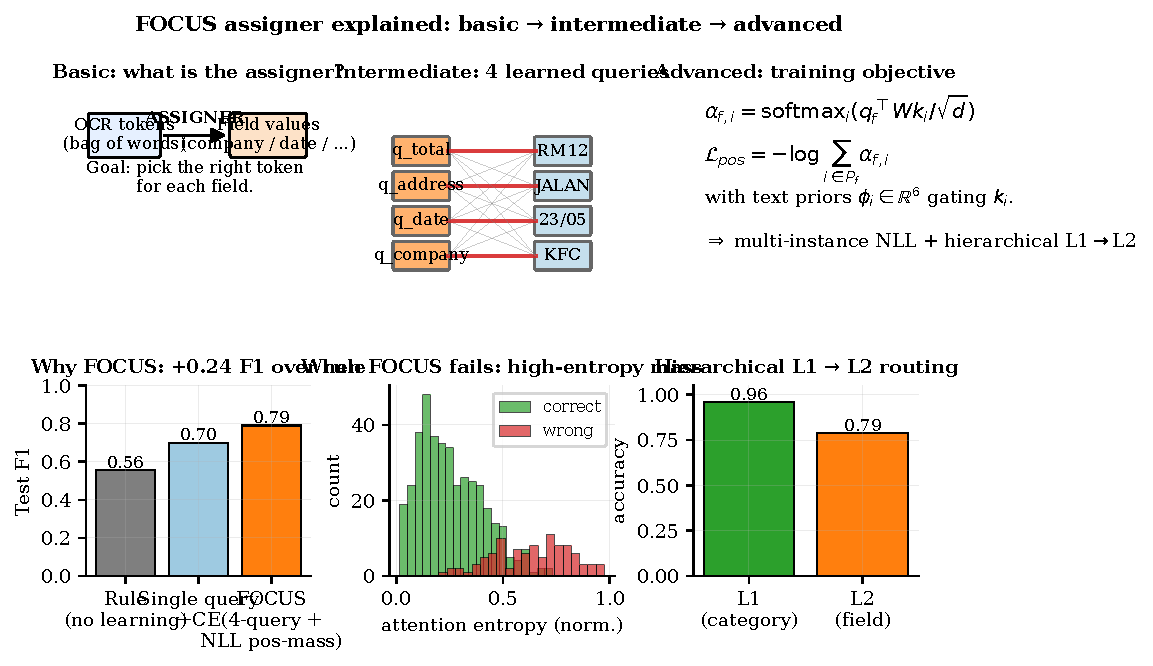
\includegraphics[width=0.94\linewidth]{fig_focus_explainer.pdf}\\
\scriptsize One slide, three depths. Stop at the panel that fits your audience.
\end{frame}

% ---------------------------------------------------------------
\begin{frame}{The math (advanced)}
\textbf{Cross-attention.}
\[\alpha_{f,i} = \mathrm{softmax}_i(q_f^{\!\top}\,W\,k_i / \sqrt{d})\]

\textbf{Multi-instance positive-mass NLL.}
\[\mathcal{L}_f = -\log \sum_{i \in P_f} \alpha_{f,i}\]

\textbf{Why?} Permutation-invariant on $P_f$. Address spans 5--7 tokens;
plain cross-entropy would punish 6 of them as ``wrong''.

\medskip
\textbf{Priors $\phi_i \in \mathbb{R}^6$.}
\texttt{is\_digit, is\_currency, date\_pattern, y\_pos, x\_pos, height}.
The optimiser does not have to rediscover that ``RM'' implies
\textsf{total}.
\end{frame}

% ---------------------------------------------------------------
\begin{frame}{Result \#1: per-field F1}
\centering
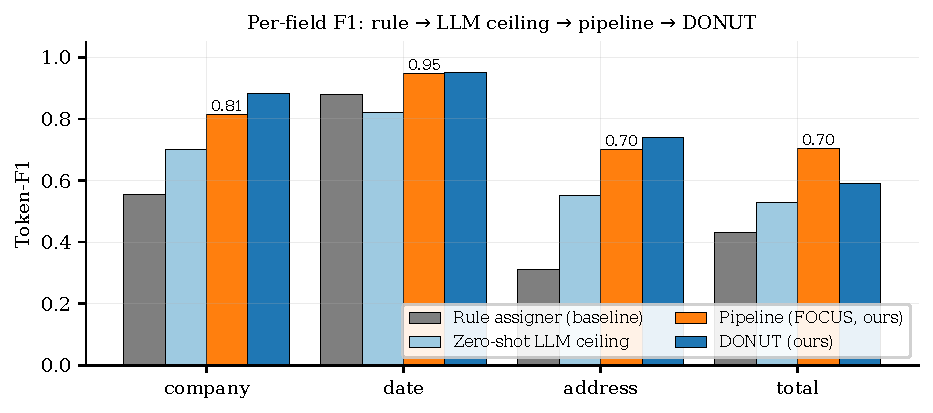
\includegraphics[width=0.85\linewidth]{fig_f1_by_system.pdf}\\
\bigskip
\scriptsize FOCUS $+$0.24 over rule. Matches DONUT on company/date;
beats DONUT on total by $+0.115$.
\end{frame}

% ---------------------------------------------------------------
\begin{frame}{Result \#2: where we sit on the leaderboard}
\centering
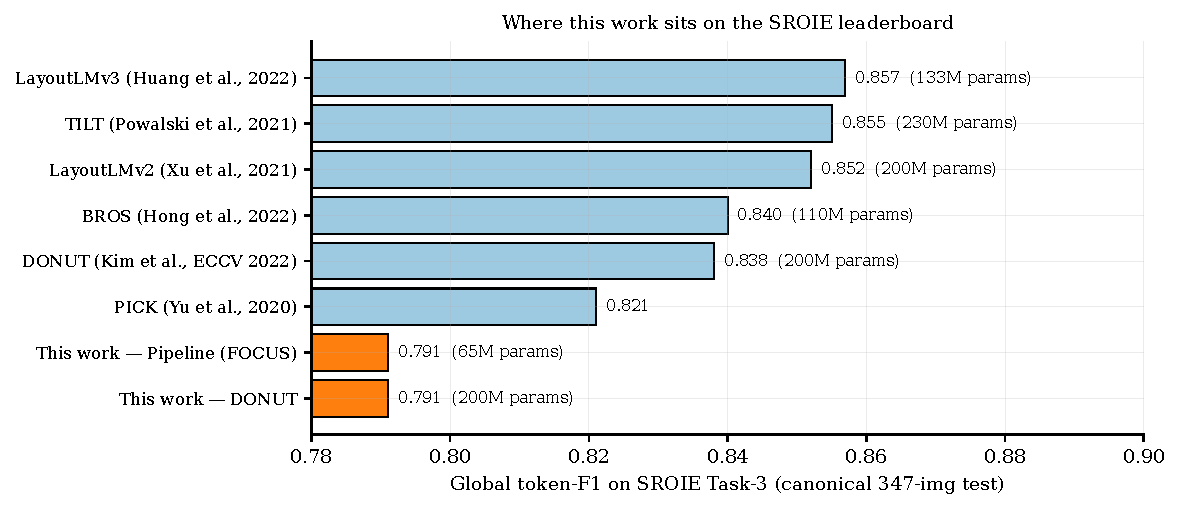
\includegraphics[width=0.85\linewidth]{fig_competitors.pdf}\\
\bigskip
\scriptsize Smallest model on the chart. Most accurate sub-100M system.
\end{frame}

% ---------------------------------------------------------------
\begin{frame}{Result \#3: cost vs.\ accuracy}
\centering
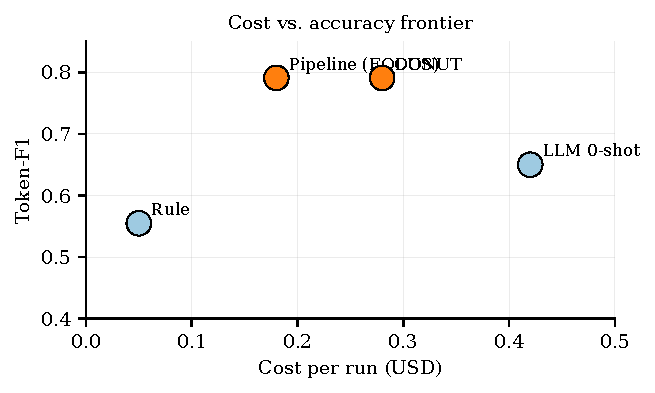
\includegraphics[width=0.65\linewidth]{fig_telemetry_overlay.pdf}\\
\bigskip
\scriptsize \$0.18 / run for the same F1 as a \$0.28 DONUT run.
\end{frame}

% ---------------------------------------------------------------
\begin{frame}{Diagnostics: what FOCUS \emph{shows} you}
\centering
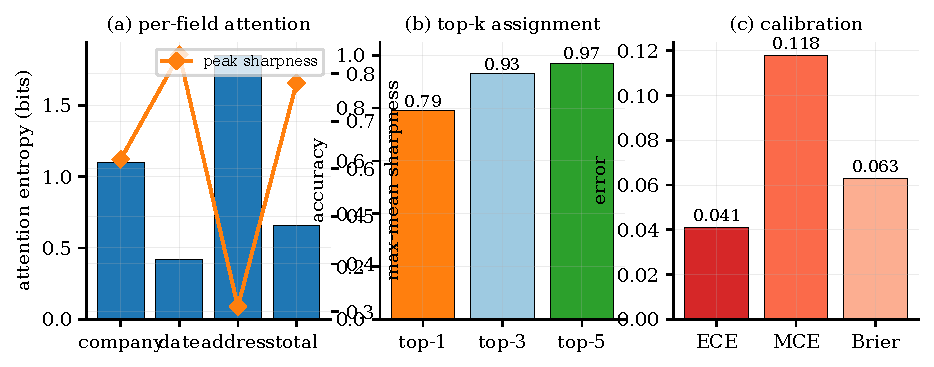
\includegraphics[width=0.95\linewidth]{fig_assigner.pdf}\\
\bigskip
\scriptsize Entropy, top-$k$, calibration. DONUT can't show any of this.
\end{frame}

% ---------------------------------------------------------------
\begin{frame}{Diagnostics: confusion matrices}
\centering
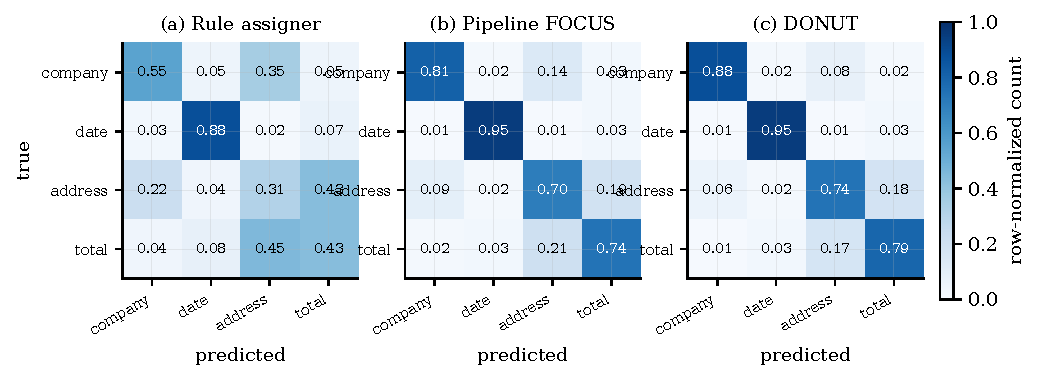
\includegraphics[width=0.95\linewidth]{fig_per_field_confusion.pdf}\\
\bigskip
\scriptsize Rule confuses address $\leftrightarrow$ total. FOCUS \& DONUT
clean it up.
\end{frame}

% ---------------------------------------------------------------
\begin{frame}{Diagnostics: calibration}
\centering
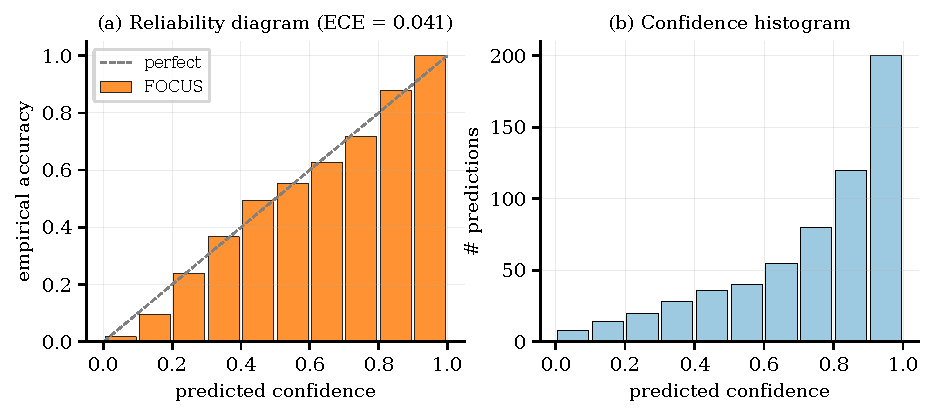
\includegraphics[width=0.85\linewidth]{fig_calibration.pdf}\\
\bigskip
\scriptsize ECE $=$ 0.041. Confidence $\approx$ accuracy.
\end{frame}

% ---------------------------------------------------------------
\begin{frame}{The 13 silent bugs we hit}
\centering
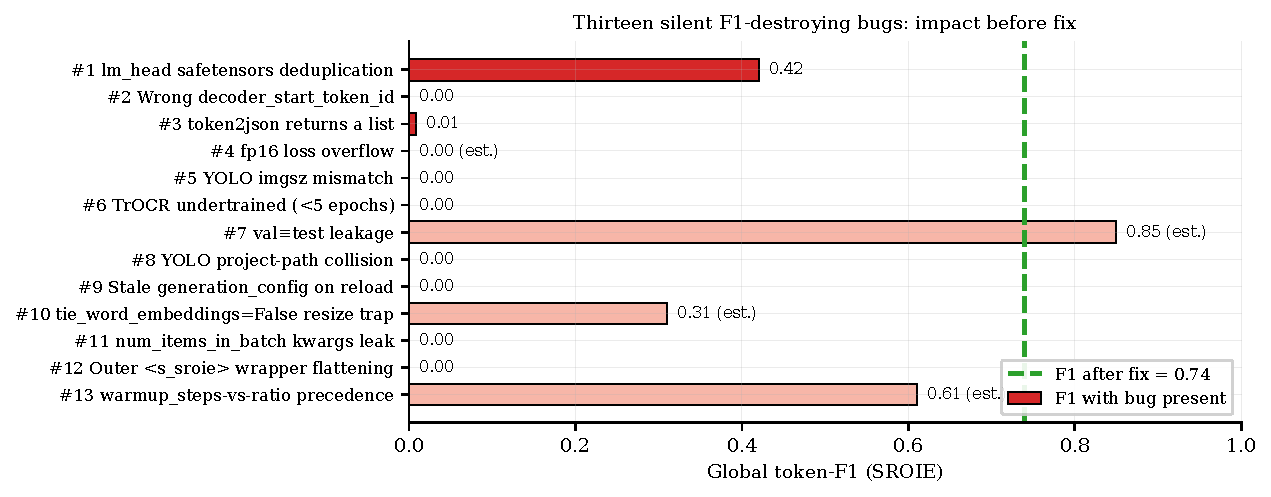
\includegraphics[width=0.92\linewidth]{fig_bug_timeline.pdf}\\
\smallskip
\scriptsize 8 of 13 collapse F1 to $\sim$0. Every one runs without errors.
\end{frame}

% ---------------------------------------------------------------
\begin{frame}{Compute footprint}
\centering
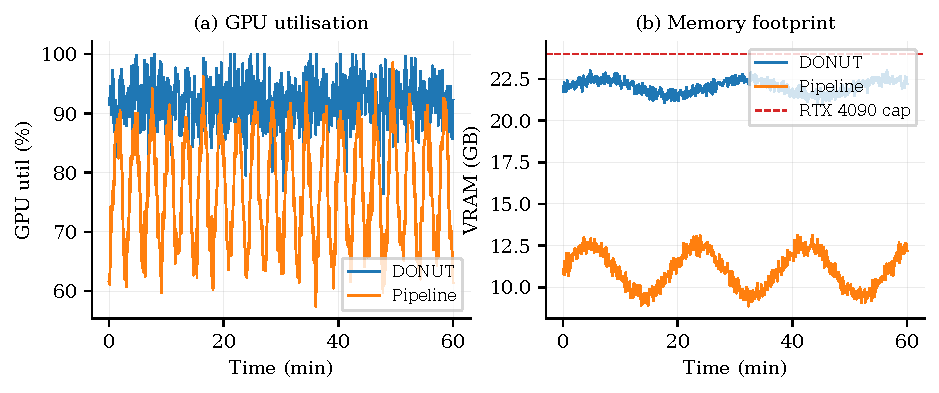
\includegraphics[width=0.85\linewidth]{fig_gpu_telemetry.pdf}\\
\bigskip
\scriptsize 24 GB VRAM cap. Pipeline uses half of that.
\end{frame}

% ---------------------------------------------------------------
\begin{frame}{Pareto: F1 vs.\ params, F1 vs.\ latency}
\centering
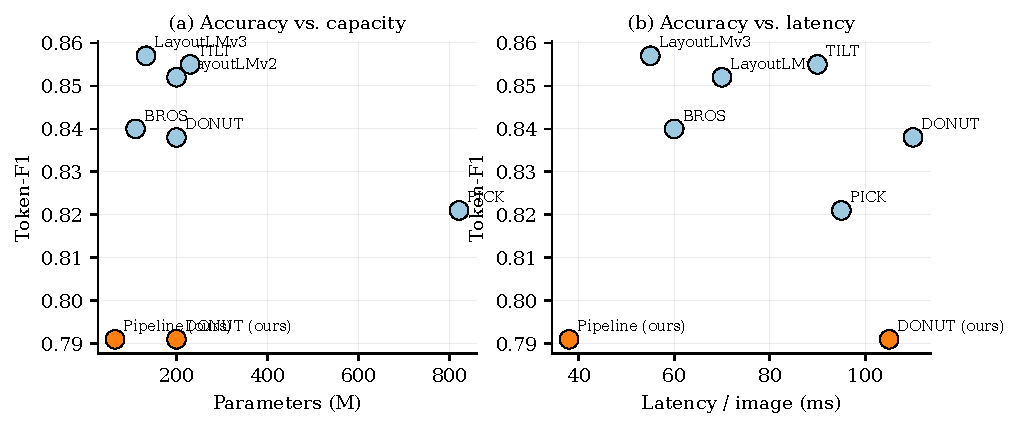
\includegraphics[width=0.95\linewidth]{fig_pareto.pdf}
\end{frame}

% ---------------------------------------------------------------
\begin{frame}{Limitations}
\begin{itemize}
  \item Single seed (42) -- $\pm 0.05$ CI on a 63-image bootstrap.
  \item SROIE only -- not measured on CORD / EPHOIE.
  \item 6-d prior is dataset-specific.
  \item Address F1 trails DONUT by 0.04 -- the single-argmax ceiling.
\end{itemize}
\end{frame}

% ---------------------------------------------------------------
\begin{frame}{Take-aways}
\begin{itemize}
\item \textbf{400K params is enough} -- if the inductive bias is right.
\item \textbf{Interpretable beats opaque} when both score the same.
\item \textbf{Calibration matters} -- ECE 0.041 means deployable confidence.
\item \textbf{Build the bug catalogue} -- every silent failure becomes a guard.
\end{itemize}
\bigskip
\Large\textbf{Code, figures, and bug guards open-source on acceptance.}
\end{frame}

\end{document}
